% Chapter Template

\chapter{Results} % Main chapter title

\label{Chapter3} % Change X to a consecutive number; for referencing this chapter elsewhere, use \ref{ChapterX}

%-------------------------------------------------------------------------------------
%	SECTION 1
%-------------------------------------------------------------------------------------
\section{Definition of Error}
To assess the degree to which changes to the analysis pipeline affect the quality of measurement, a definition of error must first be decided upon. Error is defined to be a function over pharynx space which is the difference between the intensity measured in one frame and another. The difference is divided by the average intensity of the two frames  

\[\epsilon(p) = \frac{I_{410_1}(p) - I_{410_2}(p)}{\frac{I_{410_1}(p) + I_{410_2}(p)}{2}}\]

By examining differences of intensities emitted during exposure to only 410nm, we are not affected by actual redox patterning.

\section{Collection of test data}

A large number of technical replicates were collected. A single animal was imaged 57 times in pairs of two images both at 410nm. \todo[inline]{describe conditions of image collection} It is possible that the first excitation of 410nm causes an endogenous response which would affect the fluoresence upon secondary exposure. A paired-sample t-test indicates no significant difference in the average intensity of the second image as compared to the first (p=0.41). 


%-------------------------------------------------------------------------------------
%	SECTION 2
%-------------------------------------------------------------------------------------
\section{A Partially Synthetic Dataset Increases Statistical Power}

Instead of comparing pairs of measurements taken back-to-back, we can compare all possible pairs. Given n images, we generate ${n \choose 2} = \frac{n!}{2!(n-2)!}$ pairs. This is reasonable if we do not see a change in intensity over time.

\todo{make sure this relationship is real}
\begin{figure}[ht]
    \centering
    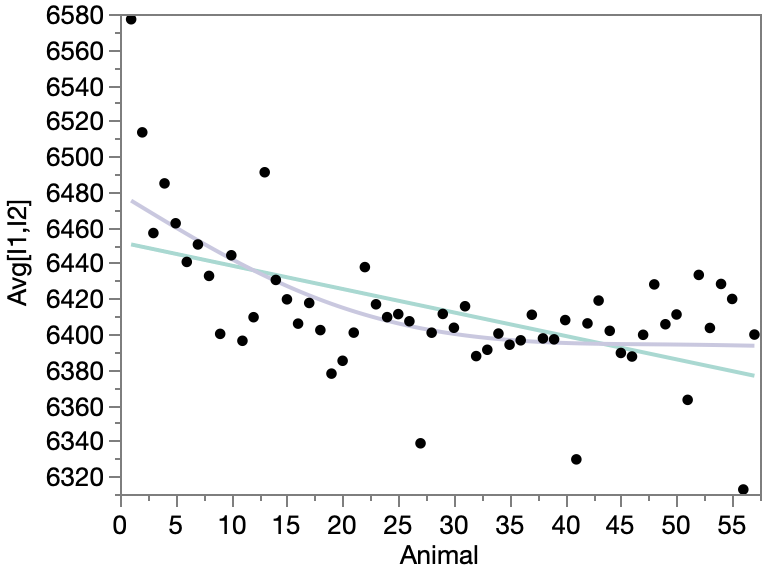
\includegraphics[scale=0.35]{Figures/rendered_files/intensity_over_time}
    \decoRule
    \caption[Average intensity over time in technical replicates]{The average intensity over time in technical replicates}
    \label{fig:DorsalVentralCartoon}
\end{figure}

%-------------------------------------------------------------------------------------
%	SECTION 3
%-------------------------------------------------------------------------------------
\section{Reductions in Manual Intervention}

\todo[inline]{show figures comparing \% requiring manual intervention for segmentation and for midlines}

%-------------------------------------------------------------------------------------
%	SECTION 4
%-------------------------------------------------------------------------------------
\section{Channel-Specific Masks and Midlines Reduce Error}

\begin{figure}[ht]
    \centering
    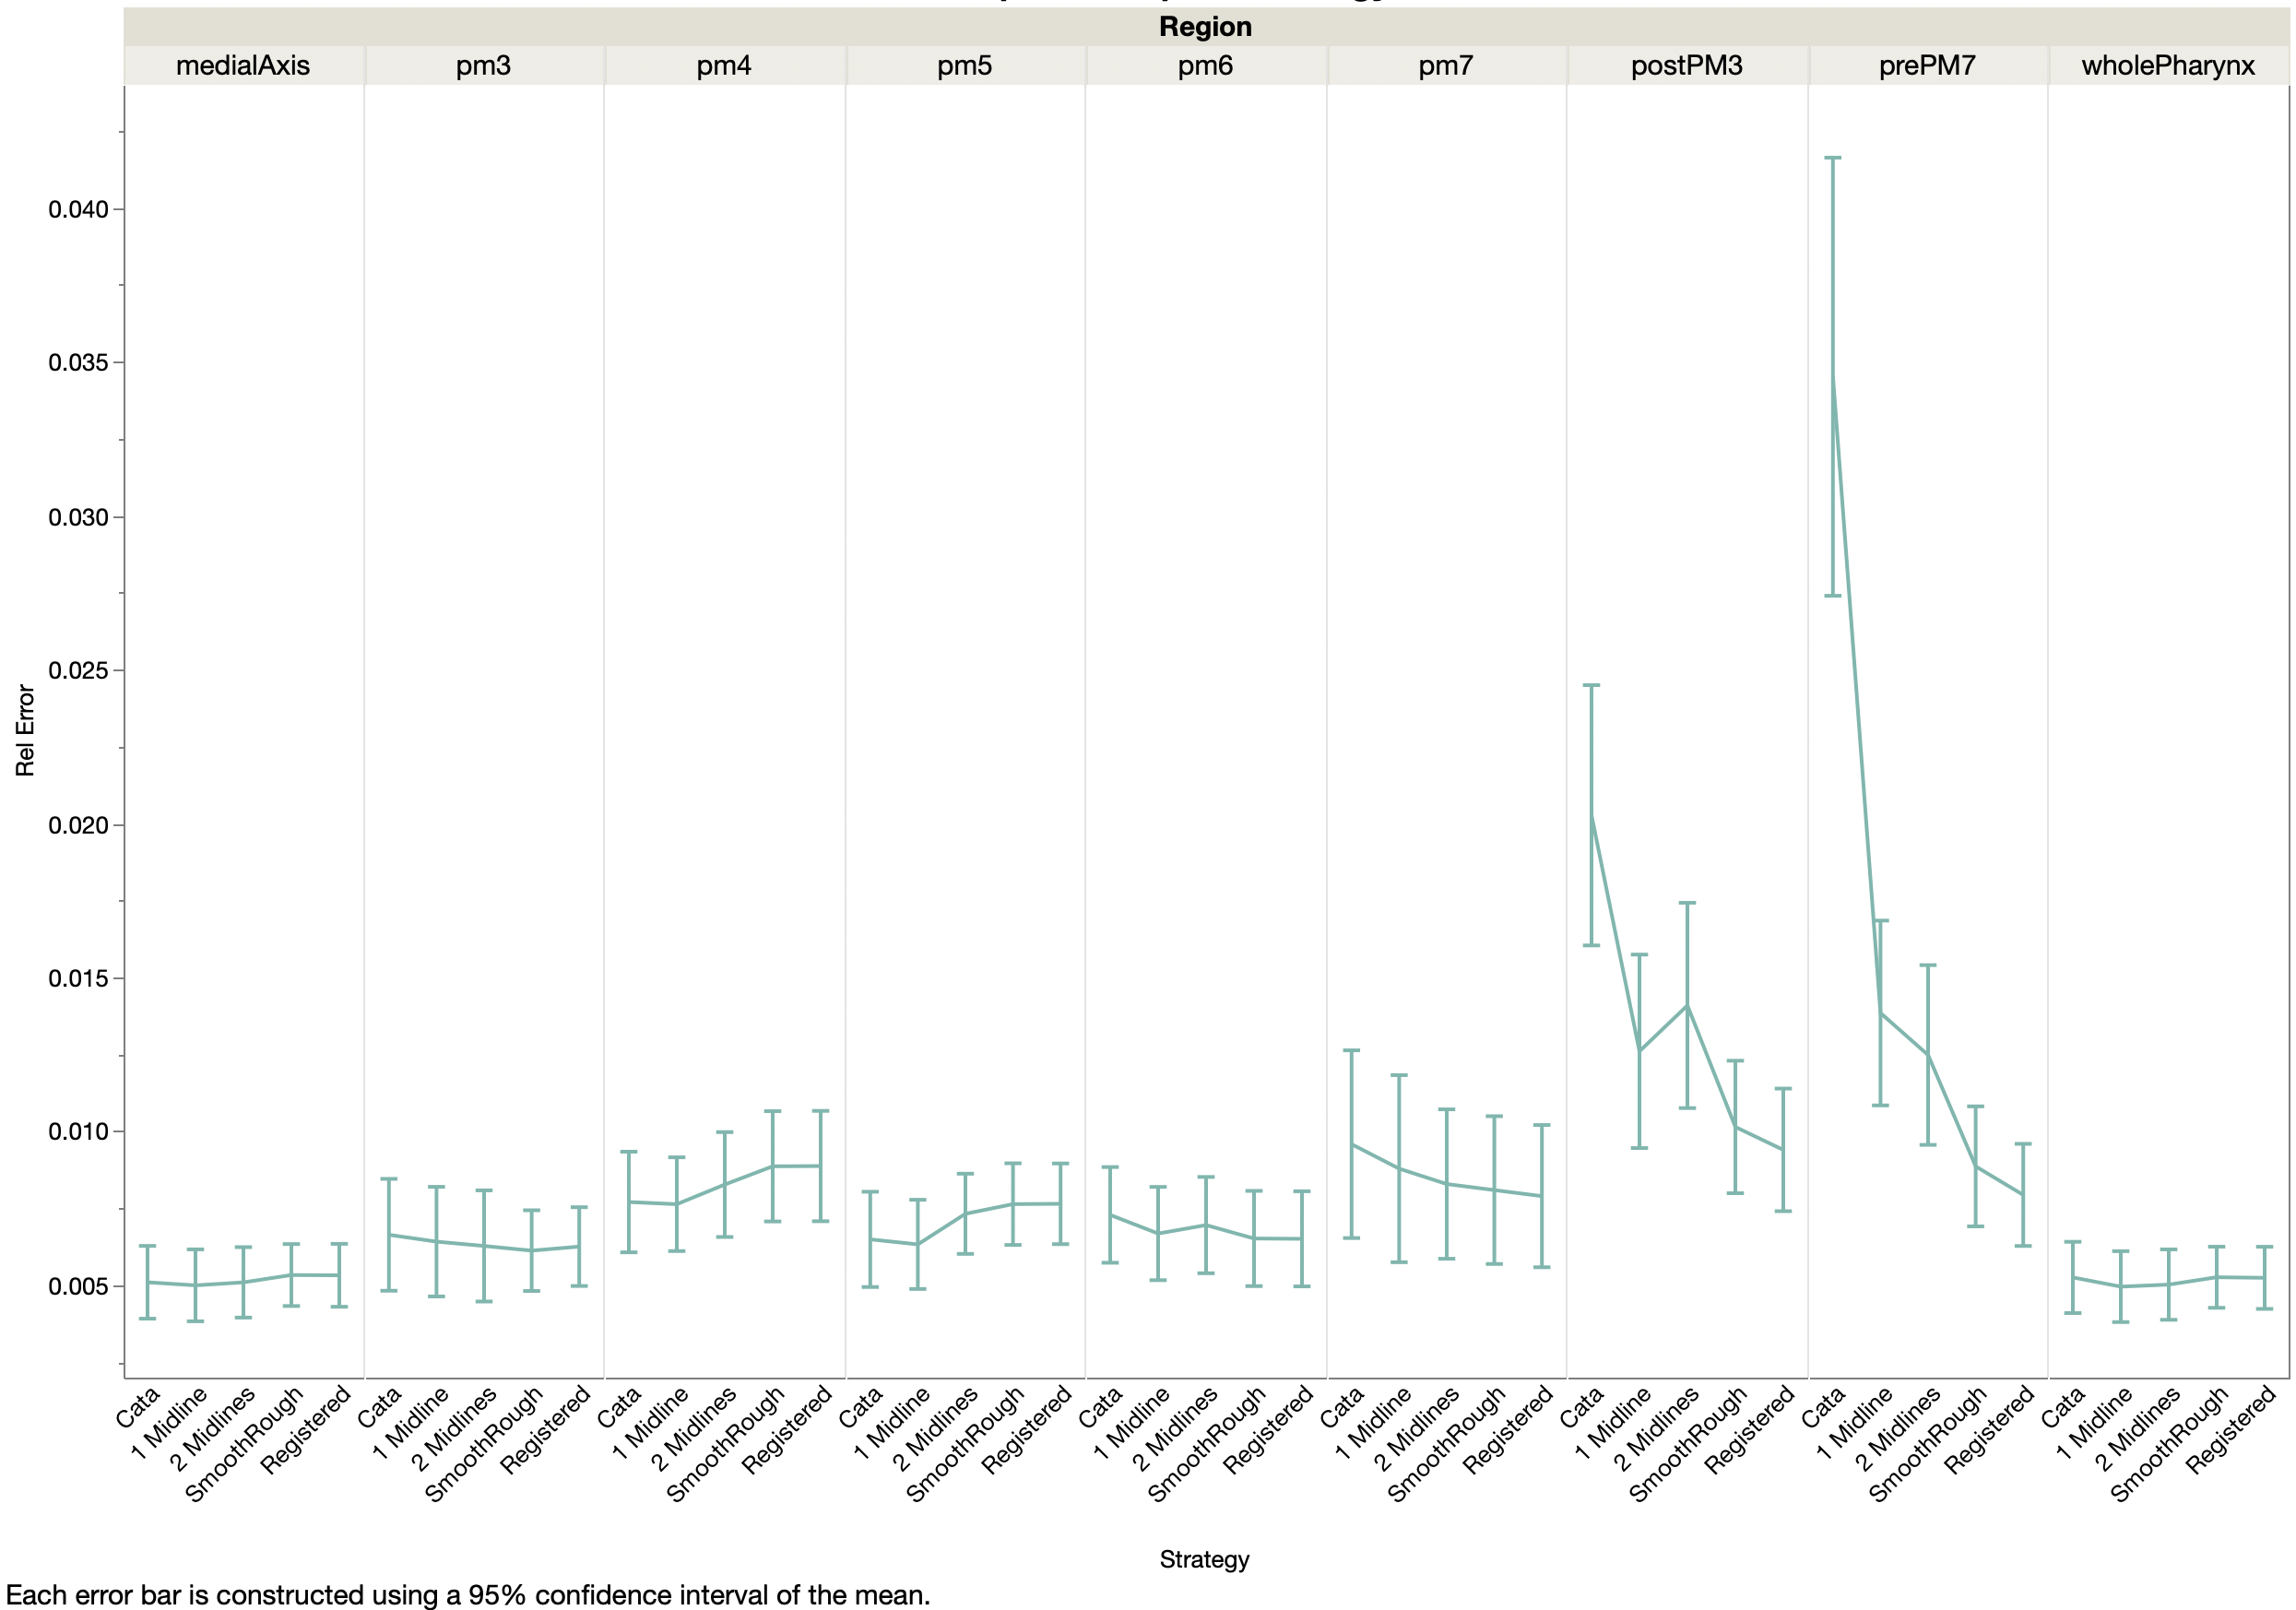
\includegraphics[scale=0.15]{Figures/rendered_files/error_by_strategy_natural}
    \decoRule
    \caption[Error by strategy in the natural data set]{Relative error}
    \label{fig:DorsalVentralCartoon}
\end{figure}

\begin{figure}[ht]
    \centering
    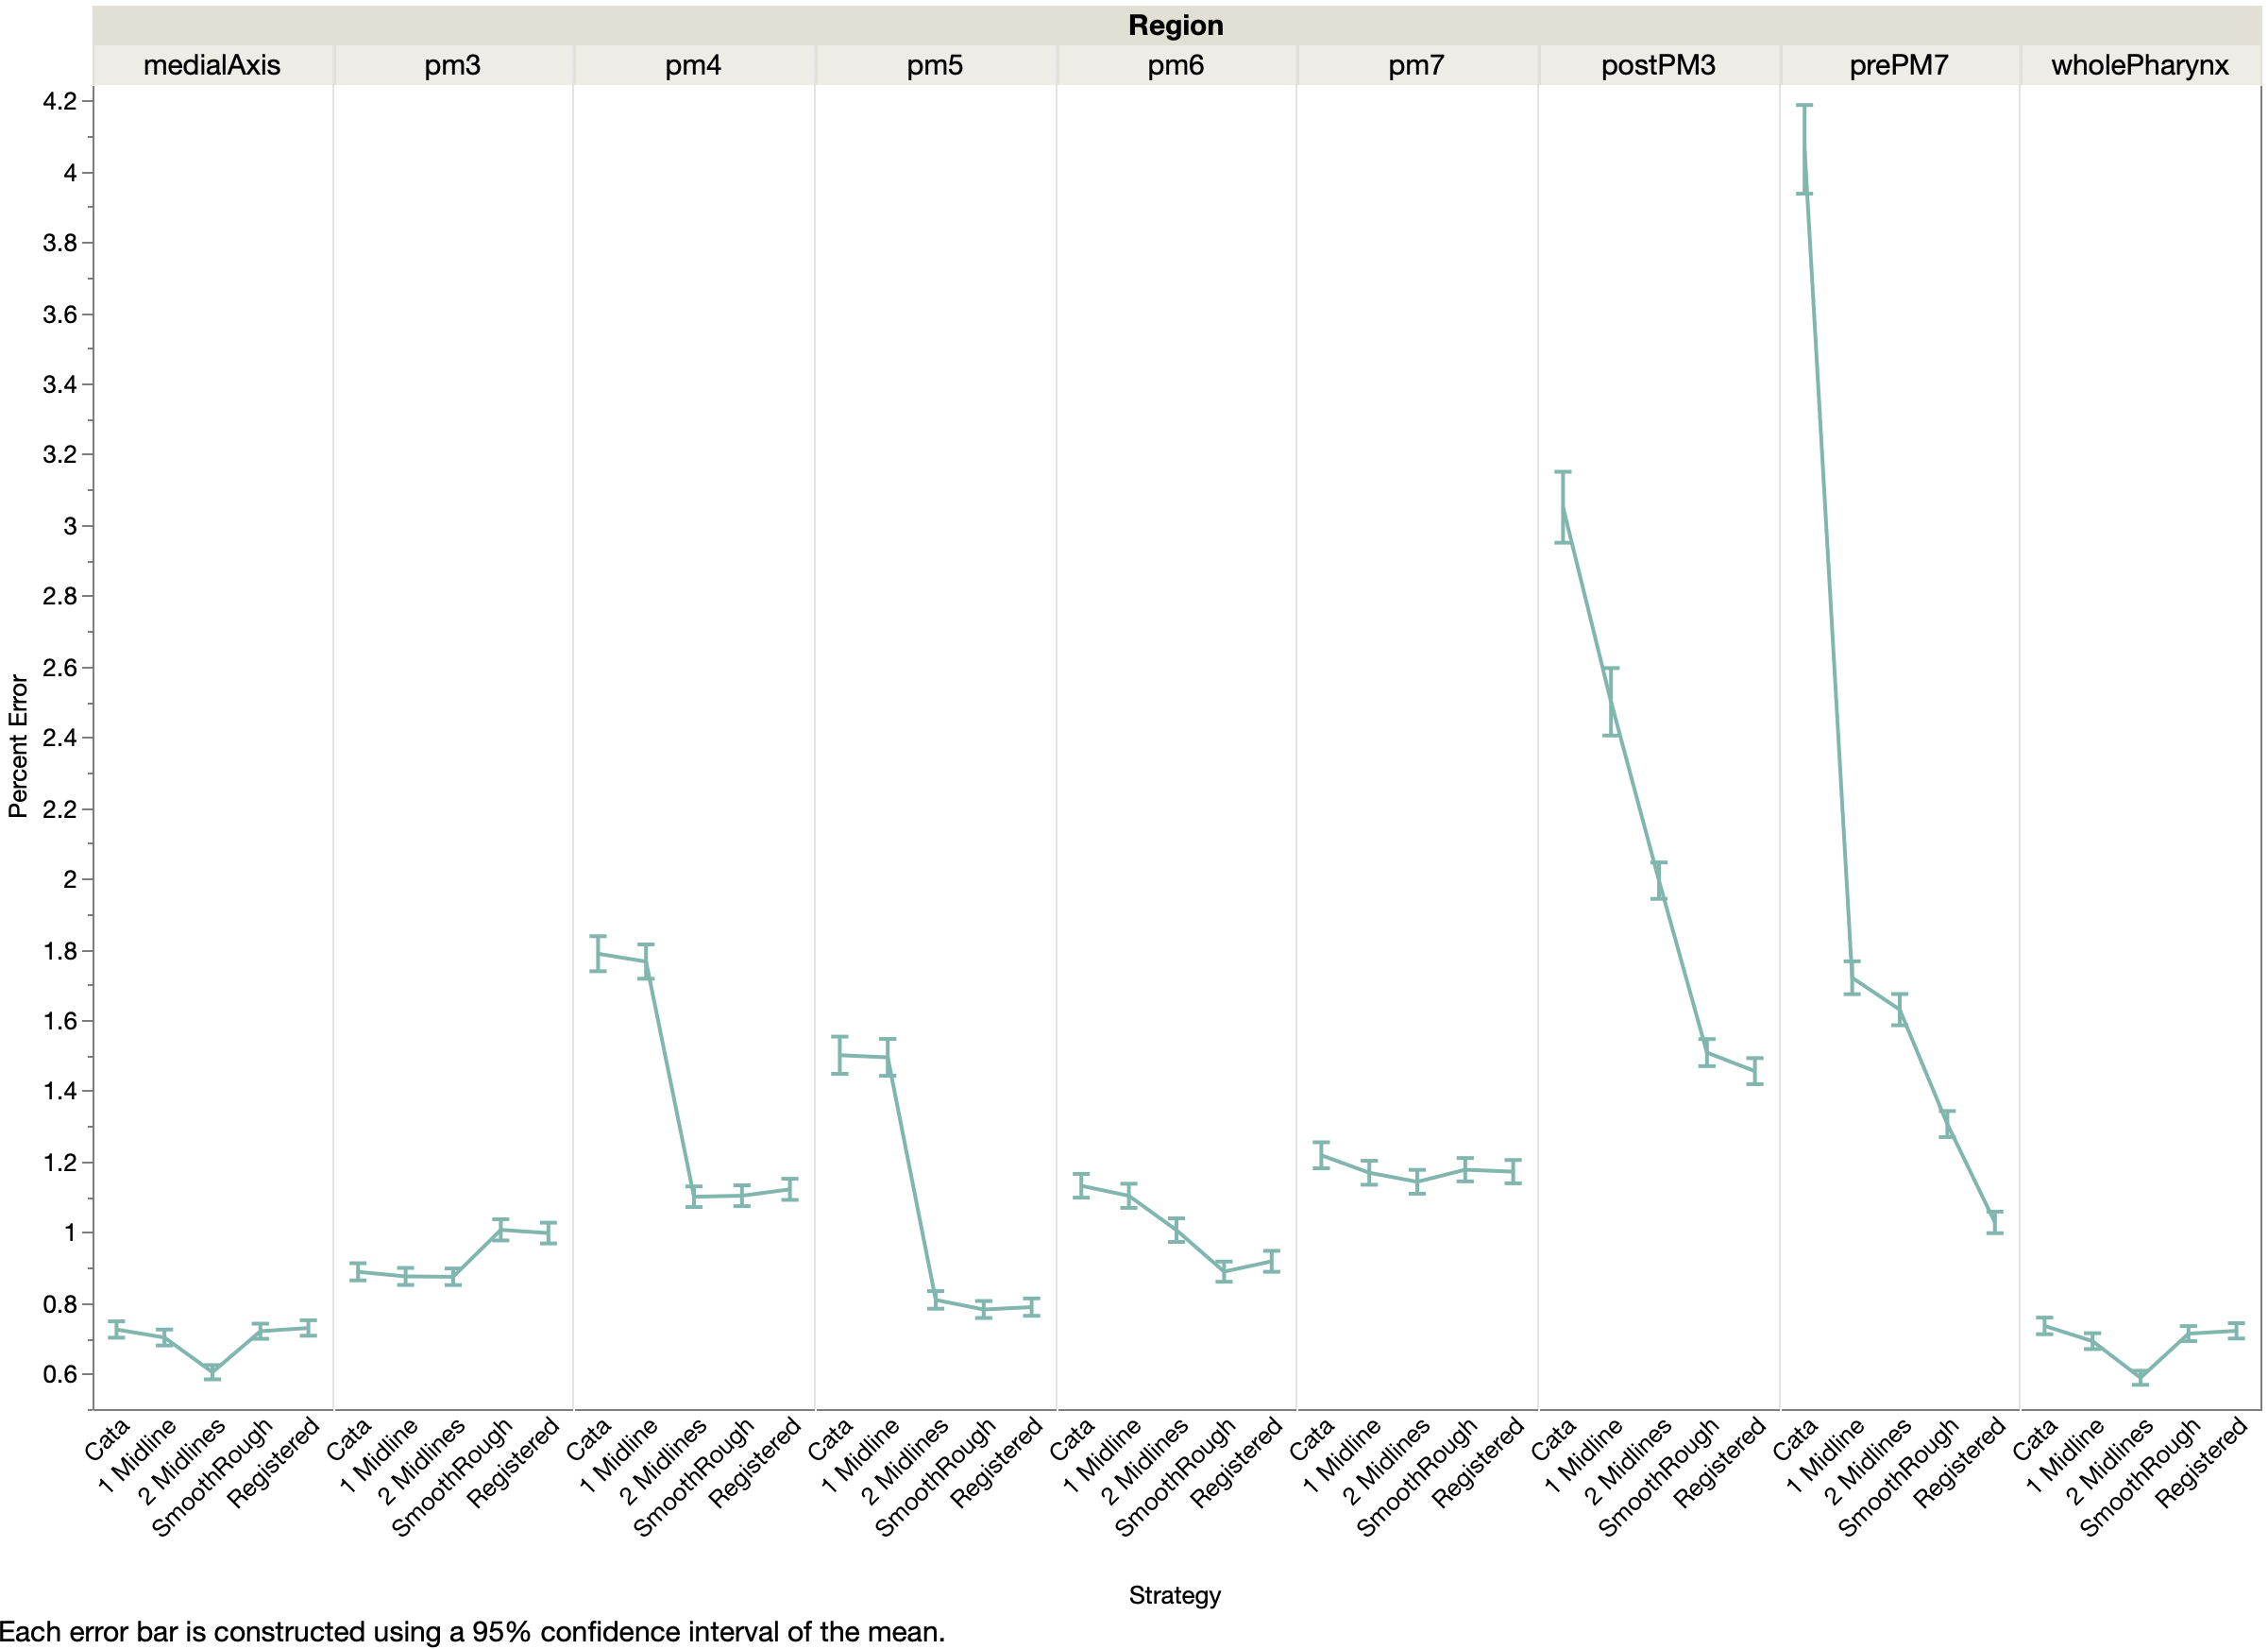
\includegraphics[scale=0.15]{Figures/rendered_files/error_by_strategy_synthetic}
    \decoRule
    \caption[Error by strategy in the synthetic data set]{}
    \label{fig:DorsalVentralCartoon}
\end{figure}